\documentclass[8pt,aspectratio=169]{beamer}
\usetheme{Madrid}
\usepackage{graphicx,booktabs,adjustbox,multicol,amsmath,amssymb,listings,xcolor}
\definecolor{mlblue}{RGB}{0,102,204}
\definecolor{mlpurple}{RGB}{51,51,178}
\definecolor{mllavender}{RGB}{173,173,224}
\definecolor{mllavender2}{RGB}{193,193,232}
\definecolor{mllavender3}{RGB}{204,204,235}
\definecolor{mllavender4}{RGB}{214,214,239}
\definecolor{mlorange}{RGB}{255,127,14}
\definecolor{mlgreen}{RGB}{44,160,44}
\definecolor{mlred}{RGB}{214,39,40}
\definecolor{mlgray}{RGB}{127,127,127}
\setbeamercolor{palette primary}{bg=mllavender3,fg=mlpurple}
\setbeamercolor{palette secondary}{bg=mllavender2,fg=mlpurple}
\setbeamercolor{palette tertiary}{bg=mllavender,fg=white}
\setbeamercolor{palette quaternary}{bg=mlpurple,fg=white}
\setbeamercolor{structure}{fg=mlpurple}
\setbeamercolor{title}{fg=mlpurple}
\setbeamercolor{frametitle}{fg=mlpurple,bg=mllavender3}
\setbeamercolor{block title}{bg=mllavender2,fg=mlpurple}
\setbeamercolor{block body}{bg=mllavender4,fg=black}
\setbeamertemplate{navigation symbols}{}
\setbeamertemplate{itemize items}[circle]
\setbeamersize{text margin left=5mm,text margin right=5mm}
\newcommand{\bottomnote}[1]{\vfill\vspace{-2mm}\textcolor{mllavender2}{\rule{\textwidth}{0.4pt}}\vspace{1mm}\footnotesize\textbf{#1}}
\usepackage{tikz,pgfplots}
\pgfplotsset{compat=1.18}
\usetikzlibrary{arrows.meta,positioning,shapes.geometric,calc}
\title{Privacy \& Zero-Knowledge Proofs: Course Preview}
\subtitle{INTRO Preview}
\author{Prof.~Dr.~Joerg Osterrieder}
\institute{University Lecture Series}
\date{\today}
\begin{document}

% Frame 1: Title
\begin{frame}
\titlepage
\end{frame}

% Frame 2: Why Zero-Knowledge Proofs Matter
\begin{frame}{Why Zero-Knowledge Proofs Matter}
\begin{columns}[T]
\begin{column}{0.62\textwidth}
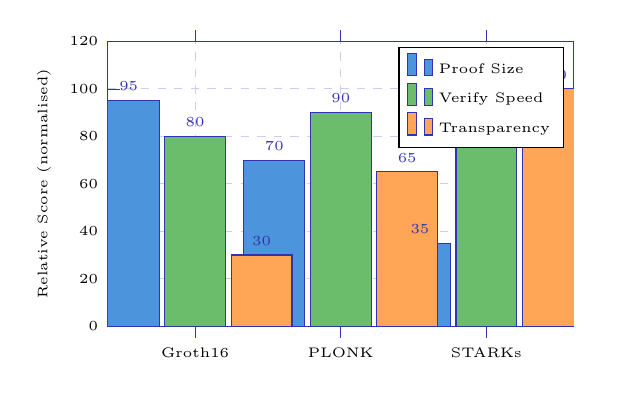
\begin{tikzpicture}
\begin{axis}[
  ybar,
  bar width=22pt,
  width=7.5cm,
  height=5.2cm,
  symbolic x coords={Groth16, PLONK, STARKs},
  xtick=data,
  xticklabels={Groth16, PLONK, STARKs},
  xticklabel style={font=\tiny, text width=2.5cm, align=center},
  ymin=0, ymax=120,
  ytick={0,20,40,60,80,100,120},
  yticklabel style={font=\tiny},
  ylabel style={font=\tiny},
  ylabel={Relative Score (normalised)},
  axis line style={draw=mlpurple},
  tick style={draw=mlpurple},
  nodes near coords,
  nodes near coords style={font=\tiny, color=mlpurple},
  point meta=y,
  enlarge x limits=0.3,
  grid=major,
  grid style={dashed, mllavender3},
  legend style={font=\tiny, at={(0.98,0.98)}, anchor=north east},
  legend cell align=left,
]
\addplot[fill=mlblue!70,   draw=mlpurple] coordinates {(Groth16,95)(PLONK,70)(STARKs,35)};
\addplot[fill=mlgreen!70,  draw=mlpurple] coordinates {(Groth16,80)(PLONK,90)(STARKs,100)};
\addplot[fill=mlorange!70, draw=mlpurple] coordinates {(Groth16,30)(PLONK,65)(STARKs,100)};
\legend{Proof Size, Verify Speed, Transparency}
\end{axis}
\end{tikzpicture}
\end{column}
\begin{column}{0.36\textwidth}
\vspace{4mm}
\begin{block}{Key Metrics}
\begin{itemize}\setlength\itemsep{4pt}
  \item[\small$\checkmark$] \small \textbf{\$10B+} ZK-rollup TVL in 2025
  \item[\small$\checkmark$] \small \textbf{$<$10ms} proof verification on-chain
  \item[\small$\checkmark$] \small \textbf{\$3B+} privacy coin market cap
  \item[\small$\checkmark$] \small \textbf{100x} throughput via ZK-rollups
\end{itemize}
\end{block}
\end{column}
\end{columns}
\bottomnote{ZK proof systems trade proof size, verification speed, and trusted-setup requirements: Groth16 is compact, PLONK is universal, STARKs are transparent.}
\end{frame}

% Frame 3: ZK Proof Landscape
\begin{frame}{ZK Proof Landscape}
\vspace{2mm}
\begin{center}
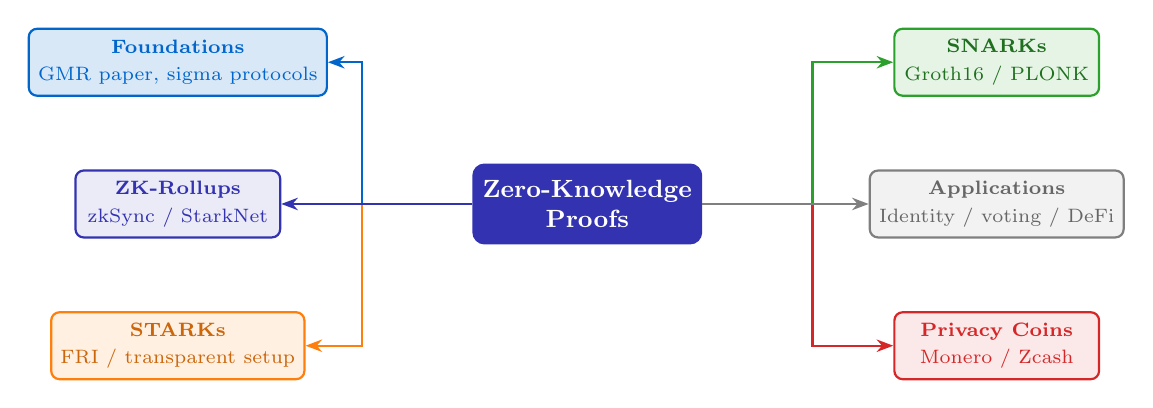
\begin{tikzpicture}[
  cbox/.style={rectangle, rounded corners=4pt, draw=mlpurple, thick,
               fill=mlpurple, minimum width=2.8cm, minimum height=1.0cm,
               font=\small\bfseries, align=center, text=white},
  sbox/.style={rectangle, rounded corners=3pt, thick,
               minimum width=2.6cm, minimum height=0.85cm,
               font=\scriptsize, align=center},
  arr/.style={-{Stealth[length=6pt]}, thick}
]
% Center node
\node[cbox] (center) at (0,0) {Zero-Knowledge\\Proofs};

% Spoke nodes
\node[sbox, draw=mlblue,   fill=mlblue!15,   text=mlblue]              (found)  at (-5.2, 1.8)
  {\textbf{Foundations}\\[2pt]GMR paper, sigma protocols};

\node[sbox, draw=mlgreen,  fill=mlgreen!12,  text=mlgreen!70!black]    (snarks) at ( 5.2, 1.8)
  {\textbf{SNARKs}\\[2pt]Groth16 / PLONK};

\node[sbox, draw=mlorange, fill=mlorange!12, text=mlorange!80!black]   (starks) at (-5.2,-1.8)
  {\textbf{STARKs}\\[2pt]FRI / transparent setup};

\node[sbox, draw=mlred,    fill=mlred!10,    text=mlred]               (priv)   at ( 5.2,-1.8)
  {\textbf{Privacy Coins}\\[2pt]Monero / Zcash};

\node[sbox, draw=mlpurple, fill=mlpurple!10, text=mlpurple]            (roll)   at (-5.2, 0.0)
  {\textbf{ZK-Rollups}\\[2pt]zkSync / StarkNet};

\node[sbox, draw=mlgray,   fill=mlgray!10,   text=mlgray!80!black]     (apps)   at ( 5.2, 0.0)
  {\textbf{Applications}\\[2pt]Identity / voting / DeFi};

% Arrows
\draw[arr, draw=mlblue]   (center.west) -- ++(-1.4,0) |- (found.east);
\draw[arr, draw=mlgreen]  (center.east) -- ++(1.4,0)  |- (snarks.west);
\draw[arr, draw=mlorange] (center.west) -- ++(-1.4,0) |- (starks.east);
\draw[arr, draw=mlred]    (center.east) -- ++(1.4,0)  |- (priv.west);
\draw[arr, draw=mlpurple] (center.west) -- ++(-1.4,0) |- (roll.east);
\draw[arr, draw=mlgray]   (center.east) -- ++(1.4,0)  |- (apps.west);
\end{tikzpicture}
\end{center}
\bottomnote{The ZK landscape spans foundational cryptography, proof system families, privacy coins, ZK-rollup scaling, and emerging applications in identity and DeFi.}
\end{frame}

% Frame 4: ZK Ecosystem Growth
\begin{frame}{ZK Ecosystem Growth}
\begin{columns}[T]
\begin{column}{0.62\textwidth}
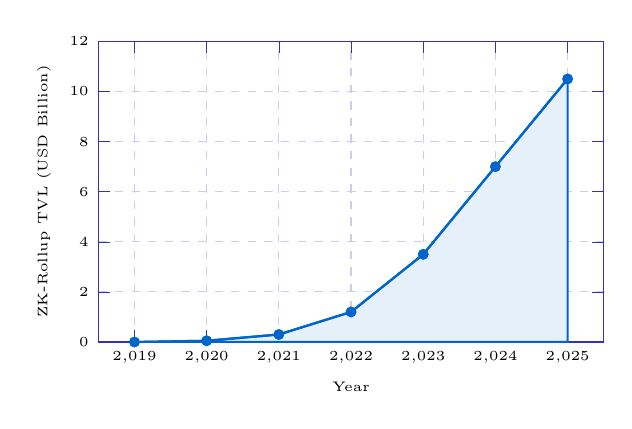
\begin{tikzpicture}
\begin{axis}[
  width=8.0cm,
  height=5.4cm,
  xmin=2018.5, xmax=2025.5,
  ymin=0, ymax=12,
  xtick={2019,2020,2021,2022,2023,2024,2025},
  ytick={0,2,4,6,8,10,12},
  xticklabel style={font=\tiny},
  yticklabel style={font=\tiny},
  xlabel style={font=\tiny},
  ylabel style={font=\tiny},
  xlabel={Year},
  ylabel={ZK-Rollup TVL (USD Billion)},
  axis line style={draw=mlpurple},
  tick style={draw=mlpurple},
  grid=major,
  grid style={dashed, mllavender3},
]
\addplot[color=mlblue, solid, thick, mark=*, mark size=1.5pt,
         fill=mlblue!10] coordinates {
  (2019,0.0)(2020,0.05)(2021,0.3)(2022,1.2)(2023,3.5)(2024,7.0)(2025,10.5)
} \closedcycle;
\addplot[color=mlblue, solid, thick, mark=*, mark size=1.5pt] coordinates {
  (2019,0.0)(2020,0.05)(2021,0.3)(2022,1.2)(2023,3.5)(2024,7.0)(2025,10.5)
};
\end{axis}
\end{tikzpicture}
\end{column}
\begin{column}{0.36\textwidth}
\vspace{4mm}
\begin{block}{Growth Drivers}
\begin{itemize}\setlength\itemsep{4pt}
  \item[\small$\checkmark$] \small \textbf{DeFi privacy} demand rising sharply
  \item[\small$\checkmark$] \small \textbf{Hardware acceleration} of proof generation
  \item[\small$\checkmark$] \small \textbf{Recursive proofs} enabling new architectures
  \item[\small$\checkmark$] \small \textbf{Regulatory pressure} boosting privacy tech
\end{itemize}
\end{block}
\end{column}
\end{columns}
\bottomnote{ZK-rollup TVL grew from near zero in 2019 to over \$10B by 2025, driven by hardware advances, recursive proving breakthroughs, and rising privacy demand.}
\end{frame}

% Frame 5: Course Coverage
\begin{frame}{Course Coverage}
\vspace{2mm}
\begin{center}
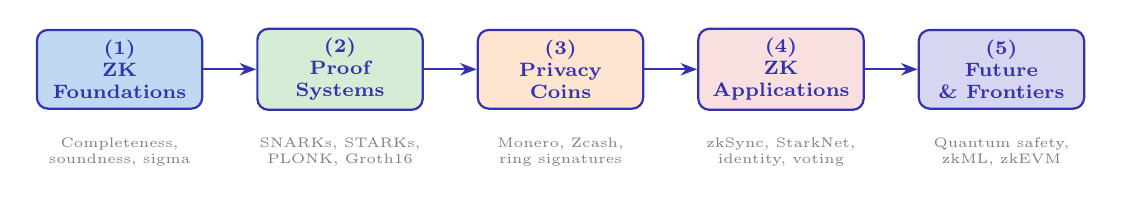
\begin{tikzpicture}[
  zkstep/.style={
    rectangle, rounded corners=4pt,
    minimum width=2.1cm, minimum height=1.0cm,
    draw=mlpurple, thick,
    fill=mllavender3,
    font=\scriptsize\bfseries,
    align=center,
    text=mlpurple
  },
  conn/.style={-{Stealth[length=6pt]}, thick, draw=mlpurple}
]
\node[zkstep, fill=mlblue!25]    (s1) at (0,0)    {(1)\\ZK\\Foundations};
\node[zkstep, fill=mlgreen!20]   (s2) at (2.8,0)  {(2)\\Proof\\Systems};
\node[zkstep, fill=mlorange!20]  (s3) at (5.6,0)  {(3)\\Privacy\\Coins};
\node[zkstep, fill=mlred!15]     (s4) at (8.4,0)  {(4)\\ZK\\Applications};
\node[zkstep, fill=mlpurple!20]  (s5) at (11.2,0) {(5)\\Future\\\& Frontiers};

\draw[conn] (s1) -- (s2);
\draw[conn] (s2) -- (s3);
\draw[conn] (s3) -- (s4);
\draw[conn] (s4) -- (s5);

\node[font=\tiny, text=mlgray, align=center, text width=2.1cm] at (0,-1.05)
  {Completeness,\\soundness, sigma};
\node[font=\tiny, text=mlgray, align=center, text width=2.1cm] at (2.8,-1.05)
  {SNARKs, STARKs,\\PLONK, Groth16};
\node[font=\tiny, text=mlgray, align=center, text width=2.1cm] at (5.6,-1.05)
  {Monero, Zcash,\\ring signatures};
\node[font=\tiny, text=mlgray, align=center, text width=2.1cm] at (8.4,-1.05)
  {zkSync, StarkNet,\\identity, voting};
\node[font=\tiny, text=mlgray, align=center, text width=2.1cm] at (11.2,-1.05)
  {Quantum safety,\\zkML, zkEVM};
\end{tikzpicture}
\end{center}
\vspace{4mm}
\begin{columns}[T]
\begin{column}{0.48\textwidth}
\begin{block}{Prerequisites}
\begin{itemize}\setlength\itemsep{2pt}
  \item[\small$\checkmark$] \small Basic cryptography and hash function knowledge
  \item[\small$\checkmark$] \small Introductory blockchain and Ethereum concepts
\end{itemize}
\end{block}
\end{column}
\begin{column}{0.48\textwidth}
\begin{block}{Outcomes}
\begin{itemize}\setlength\itemsep{2pt}
  \item[\small$\checkmark$] \small Construct and verify ZK proof arguments
  \item[\small$\checkmark$] \small Evaluate privacy coin and ZK-rollup trade-offs
\end{itemize}
\end{block}
\end{column}
\end{columns}
\bottomnote{Five modules progress from foundational ZK theory through SNARKs and STARKs to privacy coins, ZK-rollups, and the frontiers of zkML and zkEVM.}
\end{frame}

% Frame 6: What You Will Learn
\begin{frame}{What You Will Learn}
\begin{columns}[T]
\begin{column}{0.44\textwidth}
\vspace{2mm}
\begin{block}{Learning Outcomes}
\begin{itemize}\setlength\itemsep{5pt}
  \item[\small$\checkmark$] \small \textbf{Proof system mathematics} --- completeness, soundness, zero-knowledge, polynomial commitments
  \item[\small$\checkmark$] \small \textbf{SNARKs vs.\ STARKs} --- trusted setup, proof size, verification cost trade-offs
  \item[\small$\checkmark$] \small \textbf{Privacy coins} --- ring signatures, stealth addresses, shielded pools in Monero and Zcash
  \item[\small$\checkmark$] \small \textbf{ZK-rollups} --- zkSync, StarkNet architecture, sequencers, validity proofs
  \item[\small$\checkmark$] \small \textbf{ZK applications} --- private identity, on-chain voting, confidential DeFi
\end{itemize}
\end{block}
\end{column}
\begin{column}{0.54\textwidth}
\vspace{2mm}
\begin{center}
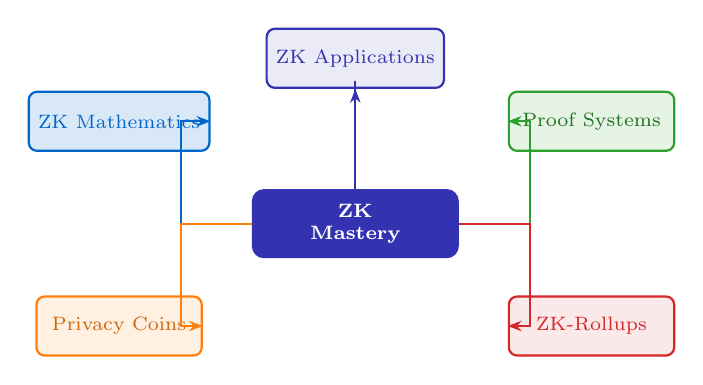
\begin{tikzpicture}[
  cbox/.style={rectangle, rounded corners=4pt, draw=mlpurple, thick,
               fill=mlpurple, minimum width=2.6cm, minimum height=0.85cm,
               font=\scriptsize\bfseries, align=center, text=white},
  fbox/.style={rectangle, rounded corners=3pt, thick,
               minimum width=2.1cm, minimum height=0.75cm,
               font=\scriptsize, align=center},
  farr/.style={-{Stealth[length=5pt]}, thick}
]
% Central node
\node[cbox] (nm) at (0,0) {ZK\\Mastery};

% Skill nodes
\node[fbox, draw=mlblue,   fill=mlblue!15,   text=mlblue]              (math) at (-3.0, 1.3) {ZK Mathematics};
\node[fbox, draw=mlgreen,  fill=mlgreen!12,  text=mlgreen!70!black]    (sys)  at ( 3.0, 1.3) {Proof Systems};
\node[fbox, draw=mlorange, fill=mlorange!12, text=mlorange!80!black]   (priv) at (-3.0,-1.3) {Privacy Coins};
\node[fbox, draw=mlred,    fill=mlred!10,    text=mlred]               (roll) at ( 3.0,-1.3) {ZK-Rollups};
\node[fbox, draw=mlpurple, fill=mlpurple!10, text=mlpurple]            (appl) at ( 0.0, 2.1) {ZK Applications};

% Arrows
\draw[farr, draw=mlblue]   (nm.west)  -- ++(-0.9,0) |- (math.east);
\draw[farr, draw=mlgreen]  (nm.east)  -- ++(0.9,0)  |- (sys.west);
\draw[farr, draw=mlorange] (nm.west)  -- ++(-0.9,0) |- (priv.east);
\draw[farr, draw=mlred]    (nm.east)  -- ++(0.9,0)  |- (roll.west);
\draw[farr, draw=mlpurple] (nm.north) -- ++(0,0.6)  |- (appl.south);
\end{tikzpicture}
\end{center}
\end{column}
\end{columns}
\vspace{1mm}
\bottomnote{By the end you will be able to reason rigorously about ZK proof systems, privacy coins, and ZK-rollup architectures from first principles to production applications.}
\end{frame}

\end{document}
